
\clearpage
\section{Das Beschaffungswesen benutzen}

Das Beschaffungswesen unterstützt den Benutzer in den Belangen von kleinen oder grossen Ausschreibungen. Das Beschaffungswesen beinhaltet beispielsweise

\begin{compactitem}
\item die Offertenerstellung,
\item die Offertenprüfung,
\item Vergabanträge,
\item Genehmigung der Vergaben und
\item die Verträge.
\end{compactitem}

\vspace{\baselineskip}

Zudem ist es möglich, verschiedene Workflows abzubilden:

\begin{compactitem}
\item Beschaffungen mit freihändiger Vergabe (mit einem Anbieter oder mehreren Anbietern).
\item Beschaffungen mit Einladungsverfahren oder offenem Verfahren.
\end{compactitem}

\vspace{\baselineskip}

Da die Workflows einer Beschaffung von Firma zu Firma oder selbst in verschiedenen Projekten ganz unterschiedlich sind, wird dieses Modul (Beschaffungswesen) jeweils auf die Prozesse eines Kunden massgeschneidert erstellt und dokumentiert. Im Folgenden werden beispielhaft Beschaffungsprozesse anhand eines möglichen Ablaufs dokumentiert und ausgeführt.

\vspace{\baselineskip}

\textbf{Einleitung:}

Um die Orientierung zu erleichtern, sind die Beschaffungen (Ausschreibungen / Offertanfragen), die Offerten und die Verträge nummeriert. Beim Erfassen dieser Elemente werden Sie jeweils aufgefordert, den Zusammenhang herzustellen (welche Offerte gehört zu welcher Beschaffung, welcher Vertrag gehört zu welcher Offerte). Die Nummerierung setzt sich dann entsprechend zusammen:

\vspace{\baselineskip}

Beschaffung Nr. 28 mit der zugehörigen Offerte Nr. 45 ergibt in der Liste der Offerten die Nummer 28.45. Wird dazu der Vertrag Nr. 31 ausgestellt, ergibt dies in der Liste der Verträge die Nummer 28.45.31. Die Nummern setzt der CUBE PA automatisch.

\vspace{\baselineskip}
\textbf{Beschaffungs- und Vertragsüberwachung auf der persönlichen Projektübersicht:}
Erreicht eine Beschaffung oder ein Vertrag einen bestimmten Status, wird die entsprechende Beschaffung oder der entsprechende Vertrag dem Benutzer auf der persönlichen Projektübersicht angezeigt. Dies ermöglicht eine rasche Übersicht über offen Aufgaben im Beschaffungswesen. Mit einem Klick wechseln Sie in die zu bearbeitende Beschaffung oder den zu bearbeitenden Vertrag (Weitere Informationen zur Konfiguration siehe Kapitel \ref{bkm:Ref20190318001}).

\subsection{Workflow für Beschaffungen mit freihändiger Vergabe}

Dieser Workflow kann für die Vergabe mit einem oder mehreren Anbietern verwendet werden. \\
Der Workflow besteht aus den folgenden Schritten:

\begin{enumerate}
\item Unterlagen für die Offertanfrage erstellen
\item Beschaffung initialisieren
\item Unterlagen für die Offertanfrage hochladen
\item Offertanfrage versenden
\item Offerte entgegennehmen und hochladen
\item Offertprüfungsprotokoll erstellen und an Entscheidungsinstanz versenden
\item Vertrag erfassen
\end{enumerate}

Für die Fortschrittskontrolle beim Bearbeiten der Beschaffungen werden Stati verwendet. Die Stati in der folgenden Tabelle beschreiben den normalen Projektfortschritt.

\vspace{\baselineskip}

\begin{tabular}{|p{5cm}|p{9.5cm}|}    % p{9.5cm} l} %{cl}  % {|m{5.316cm}|m{9.586cm}|}
\hline
\textbf{Status} & \textbf{Wer setzt den Status unter welchen Bedingungen} \\
\hline
Erstellung Ausschreibung & Dieser Status ist automatisch gesetzt, wenn eine Beschaffung initialisiert wird. \\
\hline
Freigabe Stelle X & Sie setzen den Status, sobald die Stelle X die Ausschreibung geprüft hat. \\
\hline
Versand Ausschreibung an Eingeladene & Sie setzen den Status, sobald Sie die Ausschreibung an die Anbieter versandt haben (für freihändiges Verfahren und Einladungsverfahren). \\
\hline
Offertprüfung & Sie setzten den Status, sobald Sie eine Offerte erfasst haben. \\
\hline
Offerte an Stelle X & Sie setzen den Status sobald Sie eine Offerte zusammen mit dem Offertprüfungsprotokoll an die Stelle X versandt haben. \\
\hline
Entscheid höher instanzliche Stelle & Sie setzen den Status sobald Sie eine Offerte zusammen mit dem Offertprüfungsprotokoll an die Stelle X versandt haben und im Offertprüfungsprotokoll festgehalten ist, dass beispielsweise ein Entscheid durch ein politisches Organ erforderlich ist. \\
\hline
\end{tabular}

\begin{tabular}{|p{5cm}|p{9.5cm}|}    % p{9.5cm} l} %{cl}  % {|m{5.316cm}|m{9.586cm}|}
\hline
Vergabe erfolgt & Status wird gesetzt, sobald der zuständige Projektleiter oder eine höhere Instanz der Vergabe zustimmen. \\
\hline
Vertrag ausgestellt & Die STelle X setzt den Status sobald es den Vertrag ohne Unterschrift an den Anbieter versandt hat. \\
\hline
Unterschrift Stelle X/Versand & Die Stelle X setzt den Status sobald es den vom Anbieter unterschriebenen Vertrag unterschrieben hat und an den Auftragnehmer und den Gesamtleiter versandt hat. \\
\hline
Beschaffung abgeschlossen & Sie setzen den Status, sobald Sie den Vertrag erfasst haben. \\
\hline
\end{tabular}

\vspace{\baselineskip}

Die Stati in der folgenden Tabelle beschreiben einen Abbruch oder einen Halt im Projektfortschritt:

\vspace{\baselineskip}

\begin{tabular}{|p{5cm}|p{9.5cm}|}    % p{9.5cm} l} %{cl}  % {|m{5.316cm}|m{9.586cm}|}
\hline
\textbf{Status} & \textbf{Wer setzt den Status unter welchen Bedingungen} \\
\hline
Offerte(n) abgelehnt / archiviert & Sie setzen den Status, nachdem Sie von der Projektleitung erfahren haben, dass diese Offerte überhaupt nicht mehr weiter verfolgt wird. Die Projektleitung kann den Status auch selbst setzen. \\
\hline
Offerte zur Überarbeitung zurückgewiesen & Sie setzen den Status, nachdem Sie von der Projektleitung erfahren haben, dass diese Offerte zur Überarbeitung zurückgewiesen wurde. Die Projektleitung kann den Status auch selbst setzen. \\
\hline
\end{tabular}

\subsubsection{Schritt 1: Unterlagen für die Offertanfrage erstellen}

Die Unterlagen für die Offertanfrage erstellen Sie vorab mit Excel und Word, oder anderen geeigneten Programmen.

\subsubsection{Schritt 2: Beschaffung initialisieren}

\begin{wrapfigure}[2]{l}{6.5cm}   % [x] Wie manche Zeile soll sich um die Grafik "brechen"
  \vspace{-35pt}      % Grundwert war 20; mit 30 schön oben beim Text ausgerichtet
  \begin{center}
    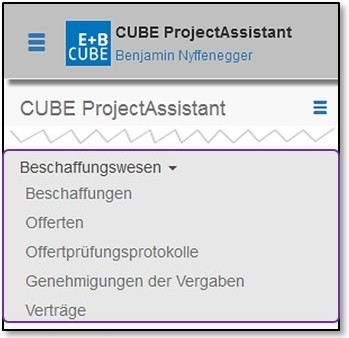
\includegraphics[width=1\linewidth]{../chapters/08_Beschaffungswesen/pictures/7-1-2_Menu_Beschaffungswesen.jpg}
  \end{center}
  \vspace{-20pt}
  \caption{Das Beschaffungswesen verwenden}
  \vspace{-10pt}
\end{wrapfigure}

Wählen Sie im Menü links den Punkt 'Beschaffungswesen' und den Unterpunkt 'Beschaffungen'. 

\vspace{10cm}

Es erscheint die Liste der Beschaffungen:

\begin{figure}[H]
\center{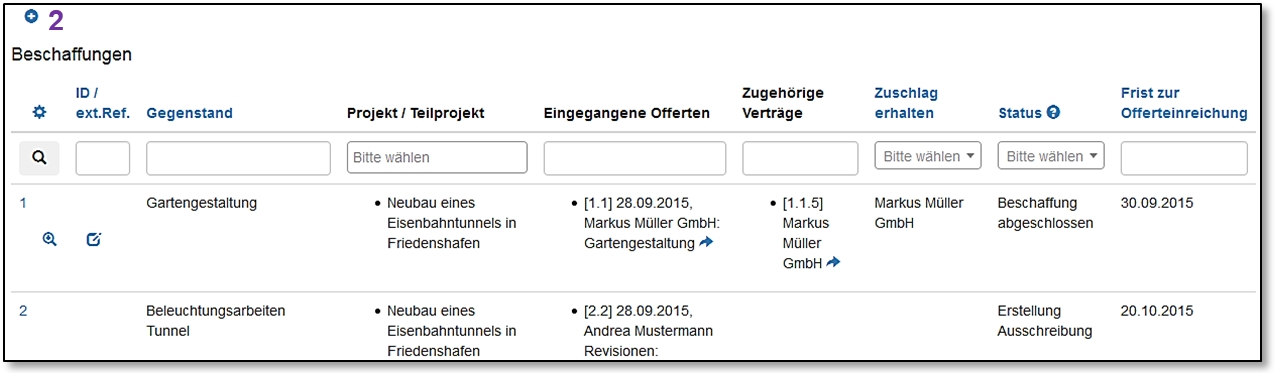
\includegraphics[width=1\linewidth]{../chapters/08_Beschaffungswesen/pictures/7-1-2_Beschaffung_Uebersicht.jpg}}
\caption{Beschaffungen Übersicht}
% \label{fig:speciation}
\end{figure}

% Problem

% \pagebreak
Klicken Sie auf das Pluszeichen 
\includegraphics[height=12pt]{/Icons/Plussymbol.jpg} \col{(2)} oben links. Es erscheint die Maske für das Erfassen neuer Beschaffungen:

\vspace{\baselineskip}

Pflichtfelder sind mit einem Stern * markiert.

\begin{figure}[H]
\center{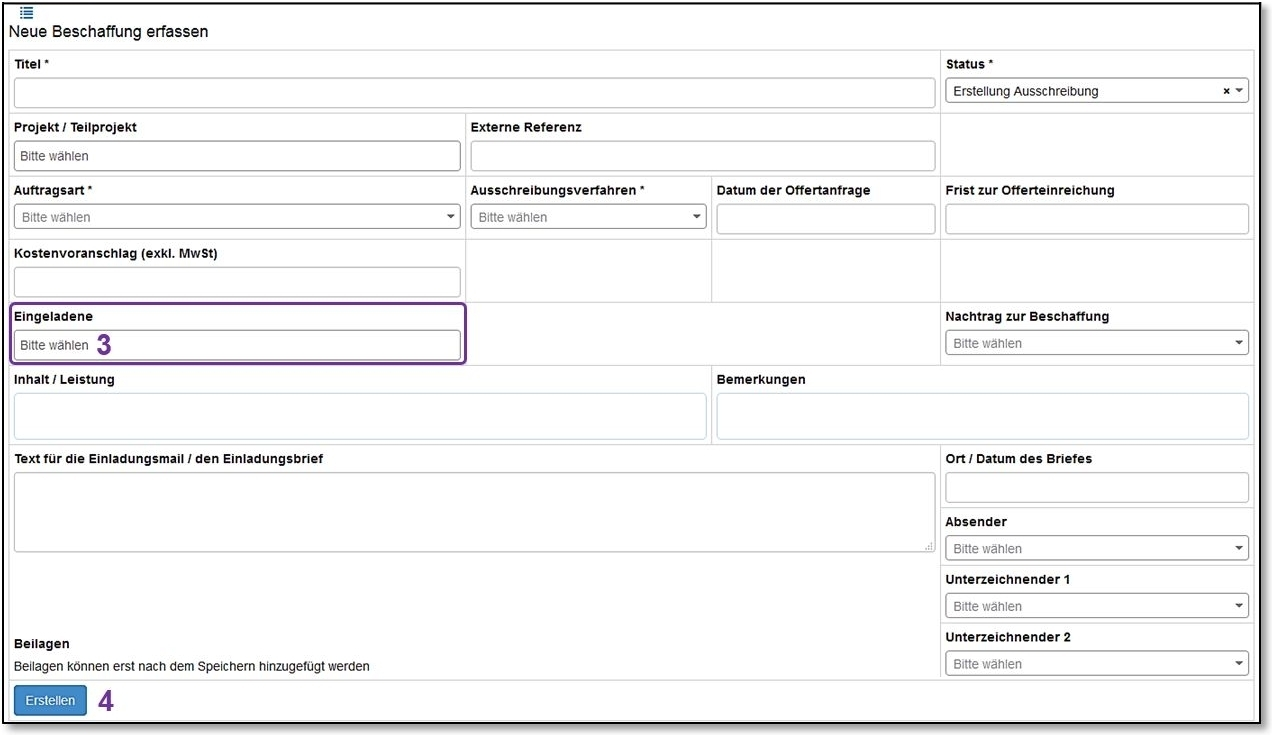
\includegraphics[width=1\linewidth]{../chapters/08_Beschaffungswesen/pictures/7-1-2_BeschaffungErfassen.jpg}}
\caption{Neue Beschaffung erfassen}
% \label{fig:speciation}
\end{figure}

Als erstes prüfen Sie, ob die Auswahlliste des Feldes 'Eingeladene' \col{(3)} die Firma enthält, an die Sie die Offertanfrage richten wollen. Falls dies nicht der Fall ist, wechseln Sie im Menü links zum Punkt 'Konfiguration' (siehe Kapitel \ref{bkm:Ref434830029}) und erfassen die Firma dort (Für diesen Schritt sind administrative Rechte notwendig. Wenden Sie sich an Ihre CUBE PA-Ansprechperson). Ist die Firma in der Auswahl vorhanden, wählen Sie sie aus. Dann können Sie die restlichen Felder ausfüllen:

\pagebreak

\begin{compactitem}
\item
Titel: Freier Text, kurz und bündig.
\item
Status: Ist automatisch auf 'Erstellung Ausschreibung' gesetzt und soll so bleiben.
\item
Projekt/Teilprojekt: wählen Sie ein oder mehrere zugehörige Projekt(e)/Teilprojekt(e).
\item
Externe Referenz: Dieses Feld wird nur für das nachträgliche Erfassen von Beschaffungen benötigt, die in der alten Beschaffungsliste vermerkt waren $\rightarrow$ nicht benutzen.
\item
Auftragsart: Wählen Sie zwischen Bauauftrag und Dienstleistungsauftrag.
\item
Ausschreibungsverfahren: Wählen Sie 'Freihändiges Verfahren'.
\item
Datum der Offertanfrage: Wählen Sie im Kalender das Datum, an dem Sie die Offertanfrage versenden.
\item
Frist zur Offerteinreichung: Wählen Sie im Kalender das Datum, an dem Sie die Offerte spätestens erhalten wollen.
\item
Kostenvoranschlag: Falls ein Kostenvoranschlag vorliegt, können Sie die Summe erfassen. Als Zeichen sind nur Zahlen und ein Punkt zugelassen. Dann haben Sie später einen direkten Vergleich zum Betrag in der Offerte.
\item
Nachtrag zur Beschaffung: Falls die jetzt bearbeitete Beschaffung einen Nachtrag zu einer anderen Beschaffung darstellen soll (das kann ein Grund sein, warum nur ein Anbieter angeschrieben wird), können Sie hier diese andere Beschaffung aus der Liste auswählen.
\item
Inhalt/Leistung: kurzer Beschrieb in freiem Text der erwarteten Leistungen des Auftragnehmers, nicht mehr als 2 bis 3 Zeilen.
\item
Bemerkungen: Hier können Sie in freiem Text besondere Umstände rund um die Beschaffung festhalten, auch in späteren Schritten.
\item
Text für die Einladungsmail / den Einladungsbrief: Erfassen Sie hier den gesamten Text der Einladungsmail oder des Einladungsbriefs, mit Ausnahme von Ort, Datum, Adresse. Mit diesem Inhalt können Sie später eine vollständige Einladungsmail oder einen Einladungsbrief generieren.
\item
Falls Sie den Einladungsbrief auf Papier versenden wollen, füllen Sie auch die Felder 'Ort, Datum des Briefs' (freier Text), 'Absender' (Listenauswahl der Firma, die den Brief verschickt), 'Unterzeichnender 1' (Listenauswahl) und 'Unterzeichnender 2' (Listenauswahl). Der 'Unterzeichnende 1' ist der hierarchisch höher gestellte, falls es zwei Unterzeichner braucht.
\end{compactitem}

\vspace{\baselineskip}

\begin{wrapfigure}[4]{r}{7cm}  
  \vspace{-30pt}    
  \begin{center}
    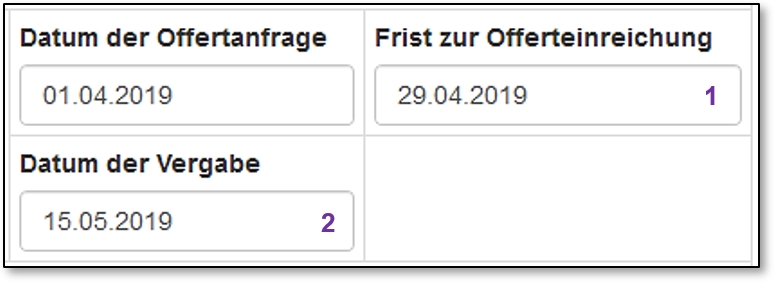
\includegraphics[width=1\linewidth]{../chapters/08_Beschaffungswesen/pictures/7-1-2_Datum_Auswahl.jpg}
  \end{center}
  \vspace{-20pt}
%  \caption{Das Beschaffungswesen verwenden}
  \vspace{-10pt}
\end{wrapfigure}

\textbf{Hinweis:} Achten Sie darauf, dass das Datum 'Frist zur Offerteinreichung' \col{(1)} vor dem 'Datum der Vergabe' \col{(2)} liegt. Andernfalls erhalten Sie eine Fehlermeldung: \textcolor{Red}{Dieser Wert ist nicht gültig.}

\vspace{\baselineskip}
\vspace{\baselineskip}

Nun klicken Sie auf die Schaltfläche 'Erstellen' \col{(4)}, darunter erscheint nun die Möglichkeit, Beilagen zu
erfassen:

\begin{figure}[H]
\center{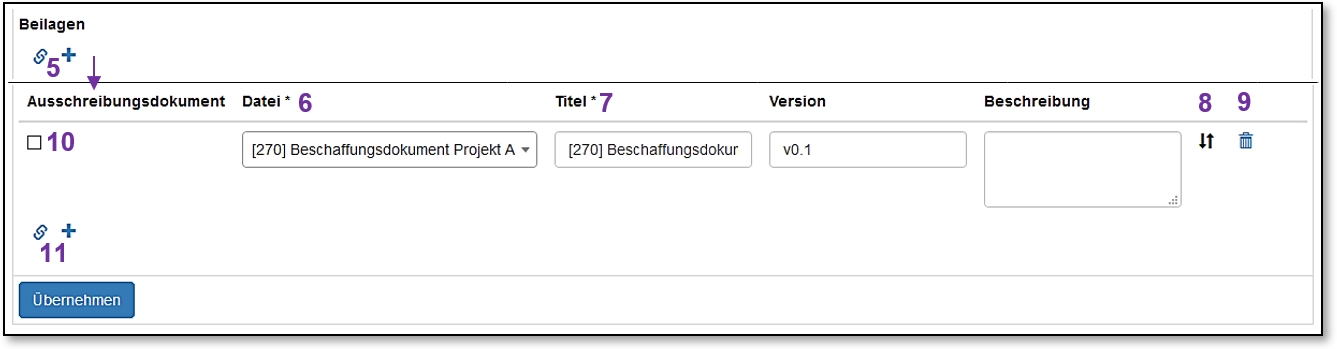
\includegraphics[width=1\linewidth]{../chapters/08_Beschaffungswesen/pictures/7-1-2_Beschaffung_Beilagen_hochladen.jpg}}
\caption{Beilagen bei Beschaffungen hochladen}
% \label{fig:speciation}
\end{figure}

Klicken Sie dazu auf das Pluszeichen 
\includegraphics[height=12pt]{/Icons/Pluszeichen.jpg} oder das Link-Symbol 
\includegraphics[height=12pt]{/Icons/Link.jpg} \col{(5)}. Nun können Sie ein bereits in CUBE PA erfasstes Dokument verknüpfen (geben Sie im Datei*-Feld \col{(6)} den Dateinamen oder Phrasen des Dateinamens des Dokuments ein) oder ein neues Dokument hochladen. Der Titel* \col{(7)} kann angepasst werden. Ergänzen Sie die weiteren Felder (Version, Beschreibung) mit den erforderlichen Angaben. Mit den Pfeilen 
\includegraphics[height=12pt]{/Icons/VertPfeile.jpg} \col{(8)} können Sie bei mehreren Beilagen die Reihenfolge ändern (Pfeile mit der linken Maustaste packen und Zeile verschieben) oder mittels dem Mülltonnensymbol 
\includegraphics[height=12pt]{/Icons/Muelltonne.jpg} \col{(9)} eine Beilage wieder löschen. sSollen die hochgeladenen Dateien für die Offertanfrage heruntergeladen werden können (beim Versand), setzen Sie das Häkchen bei 'Ausschreibungsdokument' \col{(10)}. Weitere Dokumente können mit dem 
\includegraphics[height=12pt]{/Icons/Link.jpg}-Symbol verknüpft oder mit dem \includegraphics[height=12pt]{/Icons/pluszeichen.jpg}-Symbol \col{(11)} neu hinzugefügt werden. Schliessen Sie diesen Vorgang mit 'Übernehmen' ab.

\vspace{\baselineskip}

Sie haben nun die Möglichkeit, direkt mit dem Schritt 3 weiterzufahren oder dies zu einem späteren Zeitpunkt zu tun.

\vspace{\baselineskip}

\textbf{Zwischenschritt: Eine Beschaffung nachträglich bearbeiten oder mit der Beschaffung nach einem
Unterbruch weiterfahren}

\vspace{\baselineskip}

Es ist keineswegs erforderlich, die Schritte 2 bis 4 unmittelbar hintereinander durchzuführen. Ebenso ist es möglich, nach Abschluss eines Schritts die erfassten Daten nachträglich zu ändern. Der Einstieg finden Sie immer über die Liste der Beschaffungen. Wählen Sie im Menü links den Punkt 'Beschaffungswesen' und den Unterpunkt 'Beschaffungen'. Nun erscheint die Beschaffungsliste.

\vspace{\baselineskip}

Sie können nun optisch innerhalb der gesamten Liste suchen oder die Liste filtern. Zum Blättern in der Liste scrollen Sie einfach nach unten, zuunterst sehen Sie Schaltflächen zum Blättern auf die nächste Seite, oder zum Weiter- oder Zurückblättern.

\begin{center}

\includegraphics[height=12pt]{/Icons/SeitenBlaettern.jpg}
\end{center}

Zum Filtern der Liste stehen ihnen die Suchfelder in der ersten Zeile zur Verfügung. Im Feld 'ID / ext. Ref.' Können Sie eine Zahl eingeben. Die ID ist die vom CUBE PA vergebene Laufnummer. Im Feld 'Titel' können Sie freien Text eingeben. Das Feld 'Projekt/Teilprojekt' verfügt über eine Auswahlliste. Das Feld 'Frist zur Offerteinreichung' verfügt über eine Kalenderauswahl. Haben Sie die Filterwerte ausgewählt, klicken Sie auf das Lupensymbol 
\includegraphics[height=12pt]{/Icons/Lupe_kl.jpg} \col{(1)} rechts, und die gefilterte Liste erscheint.

\begin{figure}[H]
\center{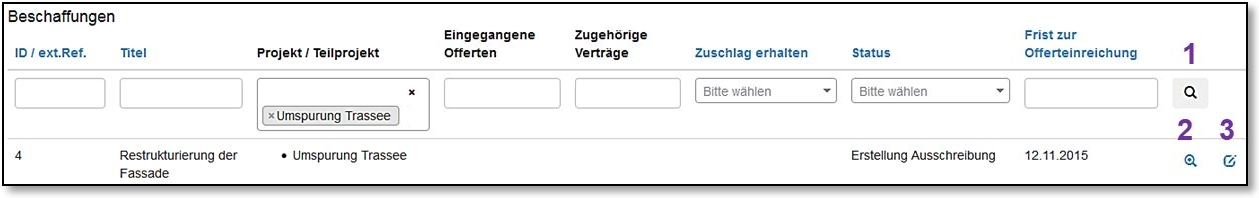
\includegraphics[width=1\linewidth]{../chapters/08_Beschaffungswesen/pictures/7-1-2_BeschaffungFiltern.jpg}}
\caption{Mit dem Filter nach Geschäften suchen}
% \label{fig:speciation}
\end{figure}

Wollen Sie einen Eintrag nur ansehen, ohne ihn zu verändern, klicken Sie auf das blaue Lupensymbol 
\includegraphics[height=12pt]{/Icons/Lupe.jpg} \col{(2)}. Der Beschaffungseintrag wird geöffnet. Wenn Sie auf das Bleistiftsymbol 
\includegraphics[height=12pt]{/Icons/Bearbeiten.jpg} \col{(3)} rechts der gesuchten Zeile klicken, öffnet sich die Maske für das Bearbeiten der Beschaffung.\textcolor{red}{ }Nun können Sie entweder vorhandene Angaben korrigieren oder zu den nächsten Schritten übergehen.

\subsubsection{Schritt 3: Unterlagen für die Offertanfrage hochladen}

Nun erfassen Sie die vorab erstellten Unterlagen für die Offertanfrage als Beilagen.

\vspace{\baselineskip}

Um eine Beilage zu erfassen, klicken Sie auf das Link-Symbol 
\includegraphics[height=12pt]{/Icons/Link.jpg} oder das Pluszeichen 
\includegraphics[height=12pt]{/Icons/Pluszeichen.jpg} \col{(1)}. Beim Verknüpfen eines Dokuments erscheinen folgende Felder: 

\begin{figure}[H]
\center{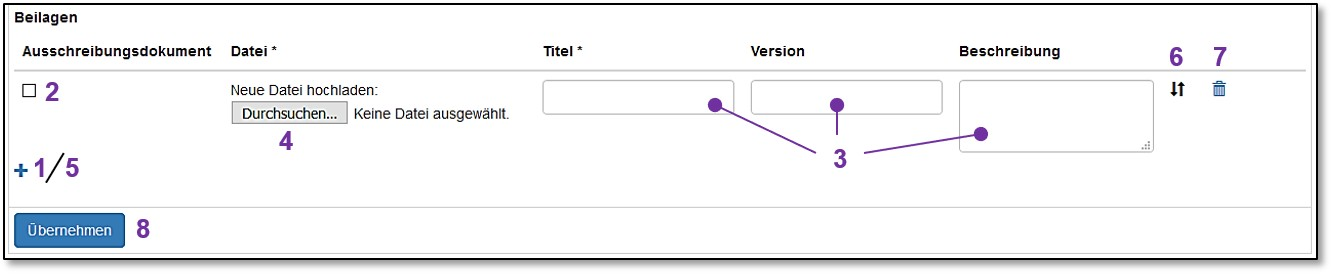
\includegraphics[width=1\linewidth]{../chapters/08_Beschaffungswesen/pictures/7-1-3_OffertanfrageHochladen.jpg}}
\caption{Eine Beilage für die Offertenanfrage hochladen}
% \label{fig:speciation}
\end{figure}

\begin{compactitem}
\item Sollen die Dokumente beim Versand heruntergeladen werden können, setzen Sie ein Häkchen bei 'Ausschreibungsdokument' \col{(2)}.
\item Titel, Version und Beschreibung sind freier Text \col{(3)}. In vielen Fällen wird es genügen, den Titel zu erfassen.
\item Geben Sie in das Titel*-Feld \col{(4)} den gesuchten Dateinamen oder Phrasen des Dateinamens ein. Sie erhalten eine Auswahl von gefundenen Dokumenten und können die exakte Version des gesuchten Dokuments verknüpfen. 
\item Mit den 
\includegraphics[height=12pt]{/Icons/Link.jpg} / \includegraphics[height=12pt]{/Icons/pluszeichen.jpg}-Symbolen \col{(5)} können weitere Beilagen verknüpft oder hochgeladen werden.
\item Sie können die Reihenfolge der Beilagen ändern, indem Sie mit der linken Maustaste ein Symbol mit den vertikalen Pfeilen 
\includegraphics[height=12pt]{/Icons/VertPfeile.jpg} \col{(6)} packen und die Zeile verschieben.
\item Durch einen Klick auf das Mülltonnensymbol 
\includegraphics[height=12pt]{/Icons/Muelltonne.jpg} \col{(7)} können Sie eine Beilage löschen.
\item Nach dem Hochladen der Beilagen und dem Bearbeiten der Angaben (Titel etc.) schliessen Sie den Vorgang mit 'Übernehmen' \col{(8)} ab.
\end{compactitem}

\vspace{\baselineskip}

\textbf{Hinweis:} Der Dateiname der hochgeladenen Beialge wird automatisch im Feld 'Titel' hinzugefügt. Sie können diesen selbstverständlich anpassen.

\subsubsection{Schritt 4: Offertanfrage versenden}

In der Maske zum Bearbeiten der Beschaffung finden Sie nun oben links ein Flieger-Symbol 
\includegraphics[height=12pt]{/Icons/Versandsymbol.jpg}. Sobald Sie darauf klicken, erscheint die Versand-Übersicht. Links steht der eingeladene Anbieter \col{(1)}, in der Mitte können Sie wiederum auf das Flieger-Symbol 
\includegraphics[height=12pt]{/Icons/Versandsymbol.jpg} \col{(2)} klicken, um eine E-Mail zu generieren, rechts können Sie auf das Briefsymbol 
\includegraphics[height=12pt]{/Icons/Briefsymbol.jpg} \col{(3)} klicken, um eine PDF-Datei des Briefs zu generieren, die sie nachher ausdrucken können.

\begin{figure}[H]
\center{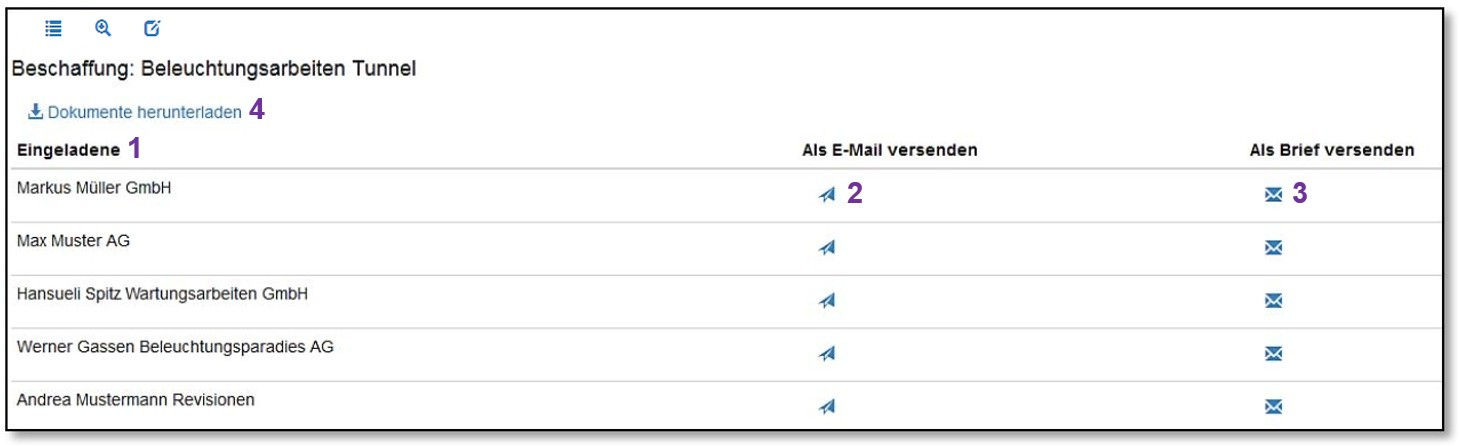
\includegraphics[width=1\linewidth]{../chapters/08_Beschaffungswesen/pictures/Besch_Versand_Uebersicht.jpg}}
\caption{Offertenanfrage versenden}
% \label{fig:speciation}
\end{figure}

Über der Versand-Übersicht befindet sich eine Schaltfläche 'Dokumente herunterladen' \col{(4)} zum Herunterladen der Beilagen. Diese benötigen Sie nur, wenn Sie die Beilagen ausdrucken und dem Brief beilegen wollen.

\vspace{\baselineskip}

Wenn sie das Fliegersymbol 
\includegraphics[height=12pt]{/Icons/Versandsymbol.jpg} anklicken, öffnet sich die generierte E-Mail in ihrem E-Mail-Programm. Kontrollieren Sie, ob Adressat, Text und Signatur korrekt sind und nehmen Sie allfällige Korrekturen vor. Die Beilagen werden dem Mail nicht beigelegt, es wird ein Link mitgeschickt, mittels dem der Empfänger die Beilagen direkt aus der Datenbank des CUBE PA herunterladen kann. Damit vermeiden Sie Probleme, die sich durch das Versenden von grossen Dateien ergeben können.

\pagebreak

\begin{wrapfigure}[7]{r}{6cm}
\vspace{-15pt}
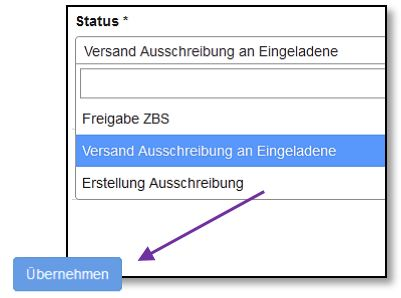
\includegraphics[height=50mm]{../chapters/08_Beschaffungswesen/pictures/7-1-4_BeschaffungEingeladene.jpg}
% \caption{Status ändern}
\end{wrapfigure}

Gehen Sie zur Liste der Beschaffungen zurück (Menü links, Punkt Beschaffungswesen, Unterpunkt 'Beschaffungen', suchen Sie die Beschaffung, öffnen Sie diese zur Bearbeitung durch einen Klick auf das Bleistiftsymbol 
\includegraphics[height=12pt]{/Icons/Bearbeiten.jpg} und setzen Sie den Status auf 'Versand Ausschreibung an Eingeladene'. Klicken Sie anschliessend auf die Schaltfläche 'Übernehmen'.



\subsubsection{Schritt 5: Offerte entgegennehmen und hochladen}

Wählen Sie im Menü links den Punkt 'Beschaffungswesen' und den Unterpunkt 'Offerten'. Es erscheint die Liste der Offerten.

\begin{figure}[H]
\center{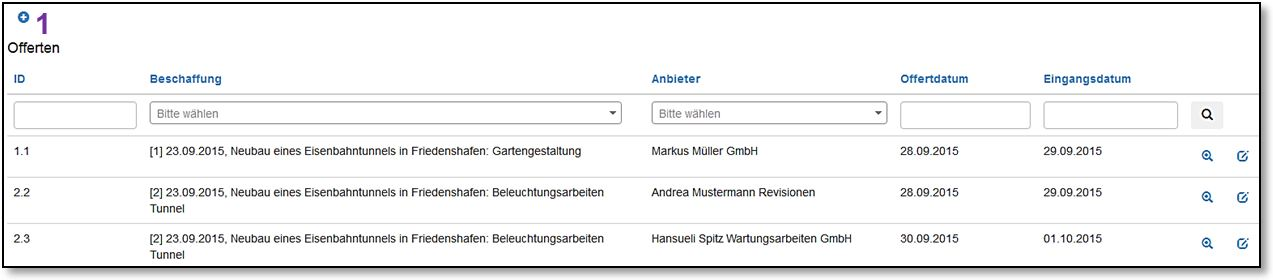
\includegraphics[width=1\linewidth]{../chapters/08_Beschaffungswesen/pictures/7-1-5_OfferteUebersicht.jpg}}
\caption{Offerten Übersicht}
% \label{fig:speciation}
\end{figure}

Klicken Sie auf das Pluszeichen 
\includegraphics[height=12pt]{/Icons/Plussymbol.jpg} \col{(1)} oben links. Es erscheint die Maske für das Erfassen neuer Offerten.

\begin{figure}[H]
\center{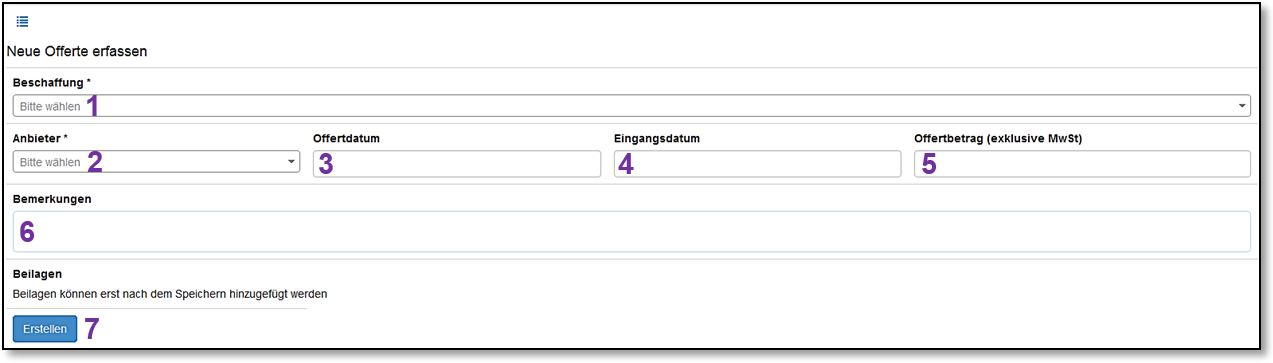
\includegraphics[width=1\linewidth]{../chapters/08_Beschaffungswesen/pictures/7-1-5_OfferteErfassen.jpg}}
\caption{Neue Offerte erfassen}
% \label{fig:speciation}
\end{figure}


Mussfelder sind mit einem Stern * markiert. Füllen Sie die Felder aus:

\vspace{\baselineskip}

\begin{compactitem}
\item
Beschaffung \col{(1)}: Wählen Sie in der Liste die 'Beschaffung' aus, zu der die Offerte gehört. \textbf{Es erscheinen nur 'Beschaffung', die den Status 'Versand Ausschreibung an Eingeladene' haben.}
\item
Anbieter \col{(2)}: Wählen Sie den Anbieter, der zur Offerte gehört. Wenn die Offertanfrage nur an einen Anbieter gesendet wurde, erscheint auch nur dieser Anbieter in der Liste.
\item
Offertdatum \col{(3)}: Mittels Kalenderauswahl setzen Sie das Datum ein, das auf der Offerte steht.
\item
Eingangsdatum \col{(4)}: Mittels Kalenderauswahl setzten Sie das Datum ein, an dem die Offerte eingetroffen ist.
\item
Offertbetrag \col{(5)}: Setzen Sie die Gesamtsumme der Offerte ein. Es sind nur Zahlen und ein Punkt gestattet.
\item
Bemerkungen \col{(6)}: Hier können Sie freien Text eintragen.
\end{compactitem}

\vspace{\baselineskip}

Klicken Sie auf die Schaltfläche 'Erstellen' \col{(7)}. Nun erscheint darunter die Möglichkeit, die Offerte
hochzuladen:

\begin{figure}[H]
\center{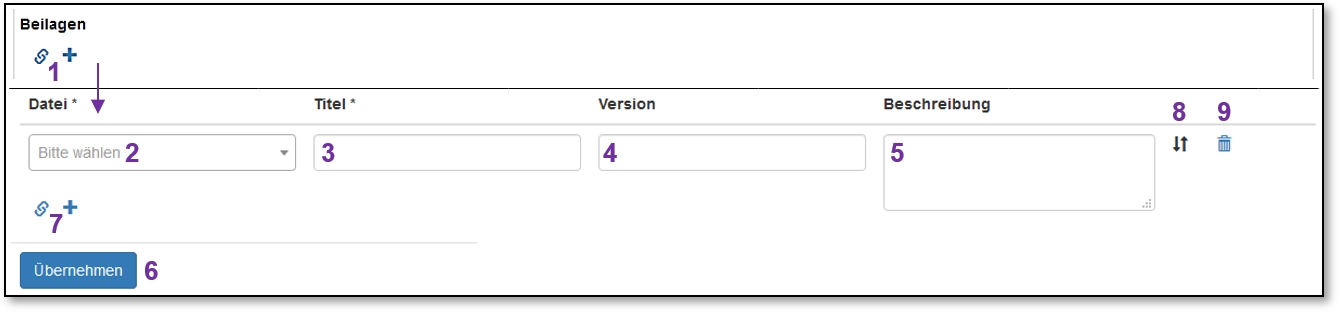
\includegraphics[width=1\linewidth]{../chapters/08_Beschaffungswesen/pictures/7-1-5_OfferteHochladen.jpg}}
\caption{Offerte hochladen}
% \label{fig:speciation}
\end{figure}

Klicken Sie auf das Link-Symbol 
\includegraphics[height=12pt]{/Icons/Link.jpg} oder das Pluszeichen 
\includegraphics[height=12pt]{/Icons/Pluszeichen.jpg} \col{(1)}, um die Offerte zu verlinken oder hochzuladen. Nach Klick auf das 
\includegraphics[height=12pt]{/Icons/Link.jpg}-Symbol \col{(1)} geben Sie in die Datei*-Zeile \col{(2)} den Namen der Offerte ein. In den meisten Fällen werden Offerten jedoch als neues Dokument mit Klick auf das 
\includegraphics[height=12pt]{/Icons/Pluszeichen.jpg}-Zeichen hochgeladen. Ein zusätzliches Fenster wird geöffnet und Sie können die Offerte im Explorer-Fenster suchen. Vergeben Sie dem Dokument die gewünschten Rechte (mindestens ein Recht muss erteilt werden) und schliessen Sie den Vorgang mit 'Erstellen' ab. Weitere Informationen zum Hochladen finden Sie in Kapitel \ref{bkm:Ref2019040401}. \\

Der Titel \col{(3)} wird vom Dateinamen übernommen, Sie können diesen jedoch anpassen. Ergänzen Sie bei Bedarf die Version \col{(4)} und die Beschreibung \col{(5)} des Dokuments als freien Text in den entsprechenden Feldern. Klicken Sie auf die Schaltfläche 'Übernehmen' \col{(6)} um die Daten zu sichern.

\vspace{\baselineskip}

Falls die Offerte aus mehreren Dokumenten besteht, klicken Sie wieder auf das Link-Symbol 
\includegraphics[height=12pt]{/Icons/Link.jpg} oder das Pluszeichen 
\includegraphics[height=12pt]{/Icons/Pluszeichen.jpg} \col{(7)} und wiederholen den Vorgang so oft wie nötig. Sie können die Reihenfolge der Dokumente verändern, indem Sie das Symbol mit den vertikalen Pfeilen 
\includegraphics[height=12pt]{/Icons/VertPfeile.jpg} \col{(8)} mit der linken Maustaste packen und die entsprechende Zeile verschieben. Mit einem Klick auf das Mülltonnensymbol 
\includegraphics[height=12pt]{/Icons/Muelltonne.jpg} \col{(9)} können Sie ein Dokument löschen.

\vspace{\baselineskip}

\begin{wrapfigure}[7]{r}{6cm}
\vspace{-15pt}
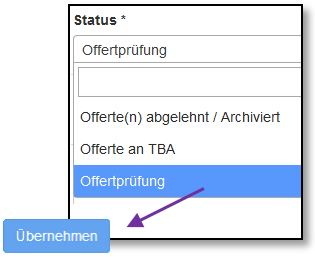
\includegraphics[height=50mm]{../chapters/08_Beschaffungswesen/pictures/7-1-5_Offertpruefung.jpg}
% \caption{Status ändern}
\end{wrapfigure}
Gehen Sie in die Liste der Beschaffungen über das Menü links, Punkt 'Beschaffungswesen', Unterpunkt 'Beschaffungen'. Suchen Sie die zur Offerte gehörende Beschaffung und setzen Sie den Status auf 'Offertprüfung', in dem Sie rechts von der Zeile auf das Bleistiftsymbol 
\includegraphics[height=12pt]{/Icons/Bearbeiten.jpg} klicken und im Feld 'Status' diesen Status anwählen. Anschliessend klicken Sie auf die Schaltfläche 'Übernehmen'.

\vspace{\baselineskip}

\textbf{Nachtragsbeschaffungen:} \\
Soll eine 'Nachtragsbeschaffung' mit einer Beschaffung verknüpft werden, wird dies innerhalb der Nachtragsbeschaffung definiert. Wechseln Sie in die Beschaffung, welche mit einer anderen Beschaffung verknüpft werden soll:

\begin{figure}[H]
\center{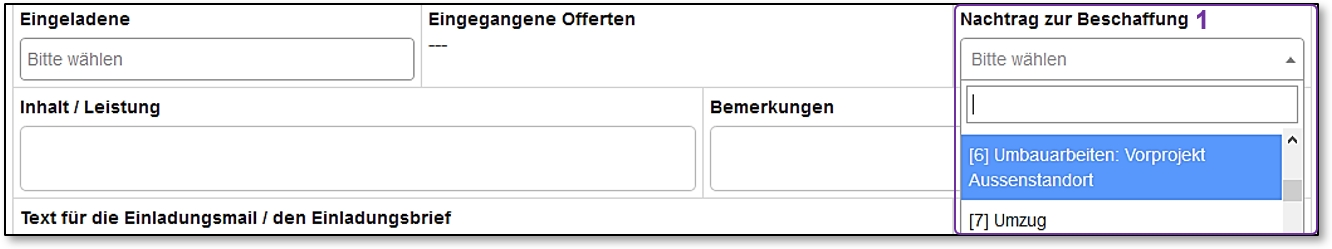
\includegraphics[width=1\linewidth]{../chapters/08_Beschaffungswesen/pictures/besch_Nachtragsbeschaffung.jpg}}
\caption{Nachtragsbeschaffung verknüpfen}
% \label{fig:speciation}
\end{figure}

Unter 'Nachtrag zur Beschaffung' \col{(1)} wählen Sie nun die (Haupt-)Beschaffung aus, mit welcher Sie die geöffnete Beschaffung verknüpfen wollen. Im Controlling-Modul (siehe Kapitel \ref{bkm:Ref20190423001}) wird das Budget einer Beschaffung ebenfalls mit dem Budget der Nachtragsbeschaffungen verknüpft.

\pagebreak

\subsubsection{Schritt 6: Offertprüfungsprotokoll erstellen und versenden}

\begin{wrapfigure}[7]{r}{6cm}
  \vspace{-30pt}      % Grundwert war 20; mit 30 schön oben beim Text ausgerichtet
  \begin{center}
    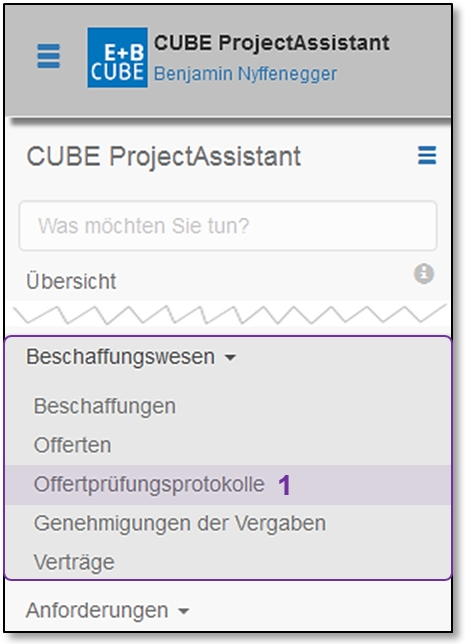
\includegraphics[height=80mm]{../chapters/08_Beschaffungswesen/pictures/7-1-6_Menu_Besch_Offertp.jpg}
  \end{center}
  \vspace{-20pt}
  \caption{Die Offertprüfungsprotokolle aufrufen}
  \vspace{-10pt}
\end{wrapfigure}

Um ein Offertprüfungsprotokoll zu erstellen und an die erforderliche Stelle zu versenden, gehen Sie wiefolgt vor: Wählen Sie im Menü links den Punkt 'Beschaffungswesen' und den Unterpunkt 'Offertprüfungsprotokolle' \col{(1)}. Es erscheint die Liste der Offertprüfungsprotokolle.

\begin{center}
\hspace{-15pt}   
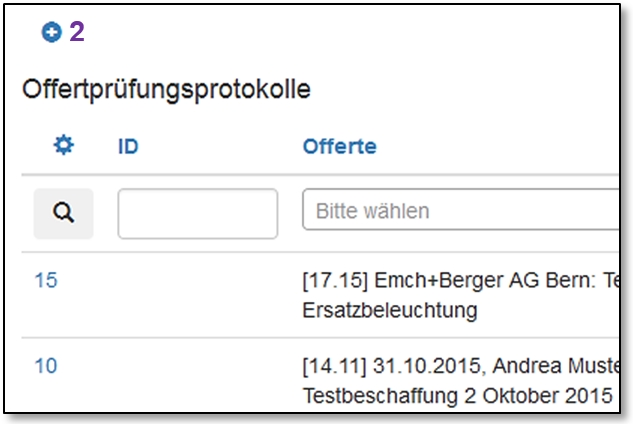
\includegraphics[width=.75\linewidth]{../chapters/08_Beschaffungswesen/pictures/7-1-6_NeuesOffertPruefProtokoll.jpg}
\end{center}

Klicken Sie auf das Pluszeichen 
\includegraphics[height=12pt]{/Icons/Plussymbol.jpg} \col{(2)} oben links. Es erscheint die Maske für das Erfassen neuer Offertprüfungsprotokolle:

\begin{figure}[H]
\center{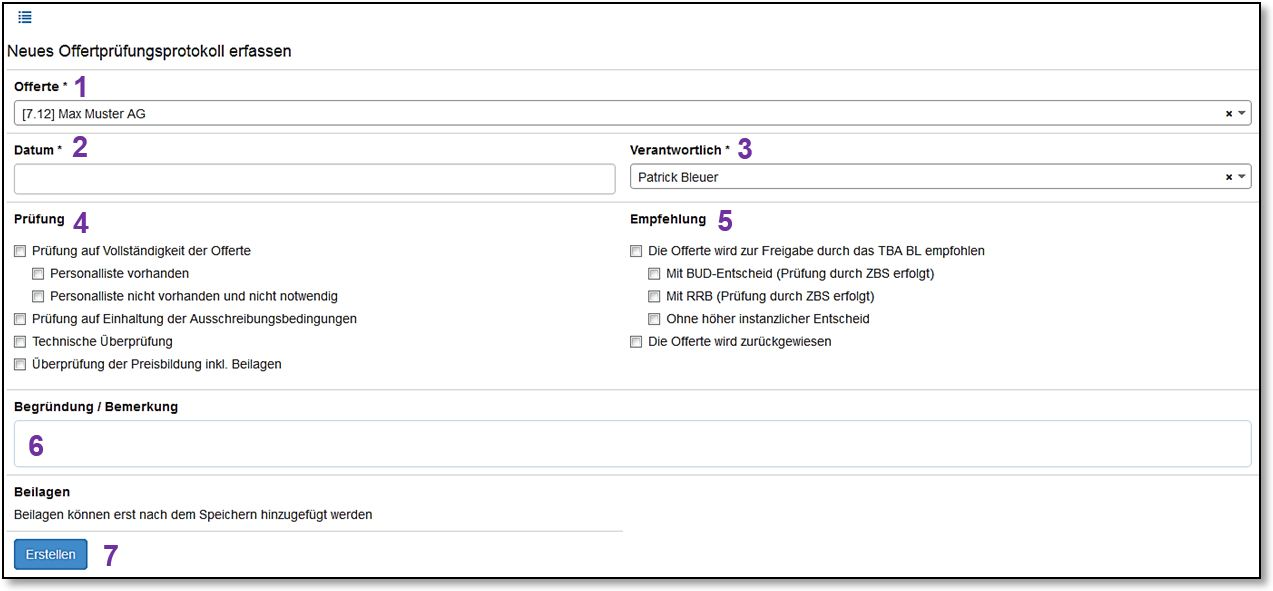
\includegraphics[width=1\linewidth]{../chapters/08_Beschaffungswesen/pictures/7-1-6_OffertpruefungsprotokollErfassen.jpg}}
\caption{Neues Offertprüfungsprotokoll erfassen}
% \label{fig:speciation}
\end{figure}

Mussfelder sind mit einem Stern * markiert. Füllen Sie die Felder aus:

\vspace{\baselineskip}

\begin{compactitem}
\item
Wählen Sie im obersten Feld die zu prüfende Offerte. Die Auswahlliste \col{(1)} zeigt nur diejenigen Offerten, für die noch kein Offertprüfungsprotokoll existiert.
\item
\textcolor{black}{Datum }\col{(2)} \textcolor{black}{: Geben Sie das Datum des Offertprüfungsprotokoll an. Beim Klicken in das Datumfeld öffnet sich ein Kalender, in welchem Sie den gewünschten Tag auswählen können. }Als Default-Wert wird jeweils das heutige Datum vorgeschlagen.
\item
Wählen Sie im Feld 'Verantwortlich' \col{(3)} den Verantwortlichen für das Offertprüfungsprotokoll aus. Der Verantwortliche ist diejenige Person, die das Offertprüfungsprotokoll unterschreibt.
\item {\sffamily
Klicken Sie unter 'Prüfung' \col{(4)} und 'Empfehlung' \col{(5)} die zutreffenden Kästchen an.}
\item
Schreiben Sie im Feld 'Begründung/Bemerkung' \col{(6)} falls nötig einen freien Text.
\end{compactitem}

\vspace{\baselineskip}

Klicken Sie auf die Schaltfläche 'Erstellen' \col{(7)}. Nun erscheint darunter die Möglichkeit, eine Beilage hochzuladen.

\begin{figure}[H]
\center{\includegraphics[width=1\linewidth]{../chapters/08_Beschaffungswesen/pictures/7-1-6_OffertenpruefungsprotokollBeilagen.jpg}}
\caption{Beilage beim Offertprüfungsprotokoll hochladen}
% \label{fig:speciation}
\end{figure}

Klicken Sie auf das Link-Symbol \includegraphics[height=12pt]{/Icons/Link.jpg} oder das Pluszeichen \includegraphics[height=12pt]{/Icons/Pluszeichen.jpg} \col{(1)}, um eine Beilage zu verlinken oder hochzuladen. Nach Klick auf das \includegraphics[height=12pt]{/Icons/Link.jpg}-Symbol \col{(1)} geben Sie in die Datei*-Zeile \col{(2)} den Namen der Beilage ein. In den meisten Fällen werden Beilagen jedoch als neues Dokument mit Klick auf das \includegraphics[height=12pt]{/Icons/Pluszeichen.jpg}-Zeichen hochgeladen. Ein zusätzliches Fenster wird geöffnet und Sie können die Beilage im Explorer-Fenster suchen. Vergeben Sie dem Dokument die gewünschten Rechte (mindestens ein Recht muss erteilt werden) und schliessen Sie den Vorgang mit 'Erstellen' ab. Weitere Informationen zum Hochladen finden Sie in Kapitel \ref{bkm:Ref2019040401}. \\

Der Titel \col{(3)} wird vom Dateinamen übernommen, Sie können diesen jedoch anpassen. Ergänzen Sie bei Bedarf die Version \col{(4)} und die Beschreibung \col{(5)} der Beilage als freien Text in den entsprechenden Feldern. Klicken Sie auf die Schaltfläche 'Übernehmen' \col{(6)} um die Daten zu sichern. Wiederholen Sie diese Schritte für weitere Beialgen.\\

Sie können die Reihenfolge der Dokumente verändern, indem Sie das Symbol mit den vertikalen Pfeilen \includegraphics[height=12pt]{/Icons/VertPfeile.jpg} \col{(7)} mit der linken Maustaste packen und die entsprechende Zeile verschieben. Mit einem Klick auf das Mülltonnensymbol \includegraphics[height=12pt]{/Icons/Muelltonne.jpg} \col{(8)} können Sie ein Dokument löschen.

\vspace{\baselineskip}

\begin{wrapfigure}[5]{r}{5cm}
\vspace{-30pt}
\includegraphics[height=40mm]{../chapters/08_Beschaffungswesen/pictures/7-1-6_OffertpruefungsprotokollPDFgen.jpg}
% \caption{Status ändern}
\end{wrapfigure}
Klicken Sie auf 'Übernehmen' \col{(6)}, um die Daten zu sichern. Nun können Sie oben links auf das
Blatt mit der gefalteten Ecke \includegraphics[height=12pt]{/Icons/BLattsymbol.jpg} klicken, um ein Offertprüfungsprotokoll als PDF-Datei zu generieren. Drucken Sie es aus und lassen Sie es unterschreiben. Das unterschriebene Dokument wird anschliessend eingescannt und bei diesem Offertprüfungsprotokoll als
Beilage wieder angehängt. Das Offertprüfungsprotokoll (Original) wird dann zusammen mit dem Papieroriginal der Offerte an die erforderliche Stelle gesendet.

\vspace{\baselineskip}

\begin{wrapfigure}[7]{r}{6cm}
\vspace{-30pt}
\includegraphics[height=50mm]{../chapters/08_Beschaffungswesen/pictures/7-1-6_BeschaffungStatus.jpg}
% \caption{Status ändern}
\end{wrapfigure}
Gehen Sie im Menü links zum Punkt 'Beschaffungswesen', Unterpunkt 'Beschaffungen'. Suchen Sie die zur Offerte gehörende
Beschaffung und setzen Sie den Status auf 'Offerte Stelle X', in dem Sie rechts von der Zeile auf das Bleistiftsymbol \includegraphics[height=12pt]{/Icons/Bearbeiten.jpg} klicken und im Feld 'Status' diesen Status anwählen. Anschliessend klicken Sie auf die Schaltfläche 'Übernehmen'.

\vspace{\baselineskip}

Nun kommen Sie erst wieder zum Zug, wenn die entsprechende Stelle den Vertrag ausgestellt hat und dieser von beiden Parteien unterschrieben wurde. Der Gesamtleiter erhält eine Kopie des Vertrags und erfasst diesen im CUBE PA, damit der Vertragsinhalt zugänglich ist.

\subsubsection{Schritt 7: Genehmigung der Vergabe durch eine höhere Instanz}

Falls Sie im Offertprüfungsprotokoll angekreuzt haben, dass die Vergabe durch eine höhere Instanz (zum Beispiel Bau- und Umweltschutzdirektion oder Regierungsrat) genehmigt werden soll, setzen Sie den Status der Beschaffung auf 'Entscheid höher instanzliche Stelle'.

\subsubsection{Schritt 8: Vertrag erfassen}

\begin{wrapfigure}[7]{r}{6cm}
  \vspace{-30pt}      % Grundwert war 20; mit 30 schön oben beim Text ausgerichtet
  \begin{center}
    \includegraphics[height=80mm]{../chapters/08_Beschaffungswesen/pictures/7-1-8_Menu_Besch_Vertraege.jpg}
  \end{center}
  \vspace{-20pt}
  \caption{Die Adressliste im Menü aufrufen}
  \vspace{-10pt}
\end{wrapfigure}

Verträge werden sowohl in TDCost erfasst (als Grundlage für die Kostenkontrolle) als auch im CUBE PA, um den Verlauf der Beschaffung vollständig zu dokumentieren und den Inhalt des Vertrags zugänglich zu machen. Erfassen Sie den Vertrag wenn möglich zuerst in TDCost, damit Sie über alle im CUBE
PA nützlichen Angaben verfügen.

\begin{center}
\hspace{-55mm}   
\includegraphics[width=.4\linewidth]{../chapters/08_Beschaffungswesen/pictures/7-1-8_NeuerVertrag.jpg}
\end{center}

\vspace{\baselineskip}

Wählen Sie im Menü links den Punkt 'Beschaffungswesen' und den Unterpunkt 'Verträge' \col{(1)}. Es erscheint die Liste der Verträge.

\vspace{\baselineskip}

Klicken Sie auf das Plussymbol \includegraphics[height=12pt]{/Icons/Plussymbol.jpg} \col{(2)} oben links. Es erscheint die Maske für das Erfassen neuer Verträge. Mit dem Listensymbol \includegraphics[height=12pt]{/Icons/Listensymbol_zurueck.jpg} \col{(3)} können Sie zurück zur Liste / Übersicht wechseln.

\begin{figure}[H]
\center{\includegraphics[width=1\linewidth]{../chapters/08_Beschaffungswesen/pictures/7-1-8_VertragErfassen.jpg}}
\caption{Neuer Vertrag erfassen}
% \label{fig:speciation}
\end{figure}

Mussfelder sind mit einem Stern * markiert. Füllen Sie die Felder aus:

\vspace{\baselineskip}

\begin{compactitem}
\item {\sffamily\color{black}
Unter 'Offerte' wählen Sie die Offerte, die als Basis zum Vertrag gedient hat. Es erscheinen nur diejenigen Offerten, die nicht zu einer abgeschlossenen Beschaffung gehören.}
\item
Der 'Vertragstitel' wird automatisch aus den Angaben zur Offerte übernommen, Sie können ihn jedoch bearbeiten.
\item
Das 'Projekt/Teilprojekt' wird automatisch aus den Abgaben zur Beschaffung übernommen. Sie können jedoch die Auswahl ändern oder ergänzen.
\item
Das 'Vertragsdatum' können Sie über eine Kalenderauswahl setzen.
\item
Das 'Startdatum' und das 'Enddatum' werden ebenso über eine Kalenderauswahl gesetzt. Es handelt sich dabei um die Termine, an denen die Leistungserbringung beginnen und enden soll.
\item
Den 'Auftraggeber' wählen Sie aus einer Auswahlliste, der 'Auftragnehmer' erscheint automatisch aufgrund der Angaben zur Offerte.
\item
Auch die 'Vertragssumme' erscheint automatisch aufgrund der Angaben zur Offerte. Sie können Sie jedoch ändern, z.B. wenn nur ein Teil der offerierten Leistungen im Vertrag enthalten sind.
\item
Die 'Vertragsnummer TDCost' erfassen Sie als freien Text, den 'Status TDCost' wählen Sie aus einer Auswahlliste. Falls Sie noch nichts in TDCost erfassen konnten, setzen Sie den Status auf 'Noch nichts erfasst'.
\item
Unter 'Überwacher' wählen Sie die Person, die für die Überwachung der Vertragsabwicklung verantwortlich ist, gleich daneben wählen Sie den / die Stellvertreter(in). \textbf{Hinweis:} Wurde ein Überwacher oder Stv. Überwacher ausgewählt und verfügt der Vertrag über einen Status, werden diese Verträge nach entsprechender Konfiguration auf der persönlichen Übersicht der Verantwortlichen aufgeführt (weitere Informationen zur Konfiguration in Kapitel \ref{bkm:Ref20190318001}).
\item
Im Feld 'Inhalt/Leistung' erscheinen automatisch die zur Offerte gehörenden Angaben, Sie können sie jedoch ändern, wenn z.B. der Vertrag nicht alle offerierten Leistungen umfasst.
\item
Im Feld 'Bemerkungen' können Sie freien Text erfassen.
\end{compactitem}

\vspace{\baselineskip}

Klicken Sie nun auf die Schaltfläche 'Erstellen' \col{(4)} und nun erscheint darunter die Möglichkeit, den Vertrag hochzuladen.

\begin{figure}[H]
\center{\includegraphics[width=1\linewidth]{../chapters/08_Beschaffungswesen/pictures/7-1-5_OfferteHochladen.jpg}}
\caption{Vertrag Hochladen}
% \label{fig:speciation}
\end{figure}

Klicken Sie auf das Link-Symbol \includegraphics[height=12pt]{/Icons/Link.jpg} oder das Pluszeichen \includegraphics[height=12pt]{/Icons/Pluszeichen.jpg} \col{(1)}, um einen Vertrag zu verlinken oder hochzuladen. Nach Klick auf das \includegraphics[height=12pt]{/Icons/Link.jpg}-Symbol \col{(1)} geben Sie in die Datei*-Zeile \col{(2)} den Namen des bereits gespeicherten Vertrags ein. In den meisten Fällen werden Verträge jedoch als neues Dokument mit Klick auf das \includegraphics[height=12pt]{/Icons/Pluszeichen.jpg}-Zeichen hochgeladen. Ein zusätzliches Fenster wird geöffnet und Sie können den Vertrag im Explorer-Fenster suchen. Vergeben Sie dem Dokument die gewünschten Rechte (mindestens ein Recht muss erteilt werden) und schliessen Sie den Vorgang mit 'Erstellen' ab. Weitere Informationen zum Hochladen finden Sie in Kapitel \ref{bkm:Ref2019040401}. \\

Der Titel \col{(3)} wird vom Dateinamen übernommen, Sie können diesen jedoch anpassen. Ergänzen Sie bei Bedarf die Version \col{(4)} und die Beschreibung \col{(5)} als freien Text in den entsprechenden Feldern. Klicken Sie auf die Schaltfläche 'Übernehmen' \col{(6)} um die Daten zu sichern. Wiederholen Sie diese Schritte falls weitere Dokumente erforderlich sind.\\

Sie können die Reihenfolge der Dokumente verändern, indem Sie das Symbol mit den vertikalen Pfeilen \includegraphics[height=12pt]{/Icons/VertPfeile.jpg} \col{(7)} mit der linken Maustaste packen und die entsprechende Zeile verschieben. Mit einem Klick auf das Mülltonnensymbol \includegraphics[height=12pt]{/Icons/Muelltonne.jpg} \col{(8)} können Sie ein Dokument löschen.

\vspace{\baselineskip}

Gehen Sie im Menü links zum Punkt 'Beschaffungswesen', Unterpunkt 'Beschaffungen'. Suchen Sie die zum Vertrag gehörende Beschaffung und setzen Sie den Status auf 'Beschaffung abgeschlossen', in dem Sie rechts von der Zeile auf das Bleistiftsymbol klicken und im Feld 'Status' diesen Status anwählen. Anschliessend klicken Sie auf die Schaltfläche 'Übernehmen'.

\vspace{\baselineskip}

\textbf{Weiteren Vertrag zu einer bestimmten Offerte erfassen.}

Wenn Sie zu einer Offerte, zu der schon einmal ein Vertrag erfasst worden ist, einen weiteren Vertrag erfassen müssen, z.B. weil eine weitere Teilleistung erbracht werden soll, suchen Sie zuerst in der Liste der Beschaffungen nach der passenden Beschaffung und falls der Status auf 'Beschaffung abgeschlossen' steht, ändern den Sie Status von 'Beschaffung abgeschlossen' auf 'Unterschrift Stelle X / Versand'. Damit stellen Sie sicher, dass Ihnen beim Erfassen des Vertrags die Offerte auch wirklich angezeigt wird. Wenn Sie den neuen Vertrag erfasst haben, setzen Sie den Status wieder auf 'Beschaffung abgeschlossen'.

\subsubsection{Eine Offerte behandeln, für die keine Offertanfrage vorhanden ist}

Es kann durchaus vorkommen, dass Sie eine Offerte erfassen müssen, für die vorher gar keine Offertanfrage versendet wurde. Zum Beispiel wurde an einer Sitzung vereinbart, dass jemand eine Offerte einreicht, oder jemand reicht eine Nachtragsofferte zu einem bestehenden Vertrag ein. In solchen Fällen gehen Sie wie folgt vor:


\begin{itemize}
\item
Initialisieren Sie eine Beschaffung so, wie unter Schritt 2 beschrieben, wobei Sie keine Inhalte erfassen müssen, die direkt mit dem Versand einer Offertanfrage zu tun haben. Falls es sich um eine Nachtragsofferte handelt, wählen Sie im Feld 'Nachtrag zu' diejenige Beschaffung, zu der die neue Offerte einen Nachtrag darstellt.
\item
Überspringen Sie die Schritte 3 und 4.
\item
Erfassen sie die Offerte so, wie unter Schritt 5 beschrieben. Dieser und die folgenden Schritte funktionieren genau gleich wie bei einer Offerte, die aufgrund einer Offertanfrage eingegangen ist.
\end{itemize}

\subsection{Workflow für Beschaffungen mit Einladungsverfahren oder offenem Verfahren}

Ein Beispiels-Workflow für Beschaffungen mit Einladungsverfahren oder offenem Verfahren folgt später.

